\documentclass[authoryear]{article}



\usepackage[T1]{fontenc}        % cesure de mots pour francais
%\usepackage[francais]{babel}    % traduction parties en francais
\usepackage{pgf}
\usepackage{pifont}
\usepackage{array}
\usepackage{topcapt}
\usepackage{float}
\usepackage[latin1]{inputenc}
 \usepackage[english]{babel}
\usepackage{amsmath,amssymb}
\usepackage{graphics}
\usepackage{graphicx}
\usepackage{dsfont}
\usepackage{booktabs}
\usepackage{tikz}
\usepackage{xcolor}
\usepackage{pifont}% http://ctan.org/pkg/pifont
\newcommand{\cmark}{\ding{51}}%


\usetikzlibrary{plotmarks}
\usetikzlibrary{arrows,backgrounds,shapes}
\tikzstyle{client}=[regular polygon,regular polygon sides=3,draw,fill=blue!50,fill opacity=1,scale=0.4]
\tikzstyle{ptf}=[draw,circle,fill=red!50,fill opacity=1,scale=0.8]
\tikzstyle{cdc}=[regular polygon, regular polygon sides=3,draw,fill=yellow!70,fill opacity=1,scale=1.2]

\tikzstyle{legend}=[scale=0.7,right,text justified]
\tikzstyle{shipment}=[->,>=stealth',blue]
\tikzstyle{ftlarc}=[->,>=stealth',very thick,red]
	\tikzstyle{vertexD}	=[circle,draw=black!80,fill=purple!70,minimum size=7pt,inner sep=0pt]
 	\tikzstyle{vertex0}	=[circle,draw=black!80,fill=purple!20,minimum size=7pt,inner sep=0pt]
 	\tikzstyle{j0}			=[circle, draw=black,fill=purple,minimum size=13pt,inner sep=0pt, scale=1]
 	\tikzstyle{farm}		=[circle, draw=black,fill=blue!80,minimum size=4pt,inner sep=0pt, scale=1]
 	
 	\tikzstyle{com2}		= [minimum size=0pt,inner sep=0pt, scale=1]
 	\tikzstyle{edgetr} 	= [draw,thick,->,purple]
 	\tikzstyle{edge1} 	= [draw,dotted,-,blue, thick]




\begin{document}
		
		\title{Two mathematical formulations of the Location Inventory Routing Problem (LIRP)}
		\author{Olivier P\'eton, Seydou Coulibaly}
		\date{\today} 
		
		\maketitle
	
%		\titlepage
 
 
    	%----------------------------------------------------------------------------------------------------  
   	
    		\section{Model 1: a "direct+loop" LIRP model}
   	   	
   	   	
     	\begin{figure}[h]
   		\centering
   		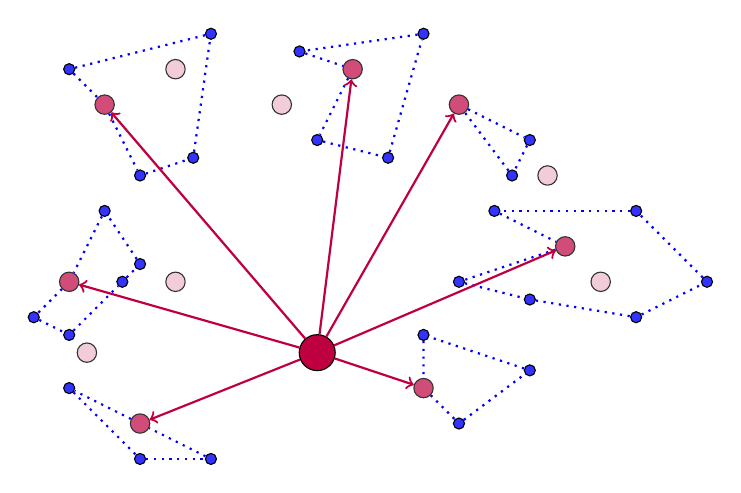
\begin{tikzpicture}[scale=0.45, auto,swap]
   		
   		\node[com2] (dum) at (0,5) {};
   		\node[j0] (j0) at (8,5) {};		
   		\node[com2] (be) at (19,5) { };
   		
   		%%%%% Collection centers   (numerotes sens horaire)
   		\foreach \pos/\name/\denom in {{(3,3)/d1}, {(1,7)/d2},  {(2,12)/d3},  {(9,13)/d4}, {(12,12)/d5}, {(15,8)/d6}, {(11,4)/d7}}
   		\node[vertexD] (\name) at \pos {$ $};
   		
   		\foreach \pos/\name/\denom in {{(1.5,5)/d91}, {(4,7)/d92},  {(4,13)/d93},  {(7,12)/d94}, {(14.5,10)/d95}, {(16,7)/d96}}
   		\node[vertex0] (\name) at \pos {$ $};
   		
   		%%%% suppliers 
   		
   		\foreach \pos/\name/\denom in {{(1,4)/f11}, {(3,2)/f12}, {(5,2)/f13}}
   		\node[farm] (\name) at \pos {$ $};
   		
   		\foreach \pos/\name/\denom in {{(1,5.5)/f21}, {(2.5,7)/f22}, {(0,6)/f23}, {(3,7.5)/f24}, {(2,9)/f25}}
   		\node[farm] (\name) at \pos {$ $};
   		
   		\foreach \pos/\name/\denom in {{(4.5,10.5)/f31}, {(1,13)/f32}, {(5,14)/f33}, {(3,10)/f34}}   	
   		\node[farm] (\name) at \pos {$ $};
   		
   		\foreach \pos/\name/\denom in {{(8,11)/f41}, {(10,10.5)/f42}, {(11,14)/f43}, {(7.5,13.5)/f44}}
   		\node[farm] (\name) at \pos {$ $};
   		
   		
   		\foreach \pos/\name/\denom in {{(14,11)/f51}, {(13.5,10)/f52}}
   		\node[farm] (\name) at \pos {$ $};
   		
   		\foreach \pos/\name/\denom in {{(14,6.5)/f61}, {(12,7)/f62}, {(17,6)/f63}, {(19,7)/f64}, {(17,9)/f65}, {(13,9)/f66}}
   		\node[farm] (\name) at \pos {$ $};
   		
   		\foreach \pos/\name/\denom in {{(14,4.5)/f71}, {(12,3)/f72}, {(11,5.5)/f73}}
   		\node[farm] (\name) at \pos {$ $};
   		
   		
   		%%% Last mile
   		\foreach \source/ \dest in {d1/f11,f11/f12,f12/f13,f13/d1}	\path[edge1] (\source) -- (\dest) ;
   		\foreach \source/ \dest in {d2/f23,f23/f21,f21/f22,f22/f24,f24/f25,f25/d2}	\path[edge1] (\source) -- (\dest) ;
   		\foreach \source/ \dest in {d3/f34,f34/f31,f31/f33,f33/f32,f32/d3}	\path[edge1] (\source) -- (\dest) ;
   		\foreach \source/ \dest in {d4/f41,f41/f42,f42/f43,f43/f44,f44/d4}	\path[edge1] (\source) -- (\dest) ;
   		\foreach \source/ \dest in {d5/f51,f51/f52,f52/d5}	\path[edge1] (\source) -- (\dest) ;	
   		\foreach \source/ \dest in {d6/f62,f62/f61,f61/f63,f63/f64,f64/f65,f65/f66,f66/d6}	\path[edge1] (\source) -- (\dest) ;
   		\foreach \source/ \dest in {d7/f72,f72/f71,f71/f73,f73/d7}	\path[edge1] (\source) -- (\dest) ;
   		
   		%%%% Routes
   		\foreach \source/ \dest in {j0/d1,j0/d2,j0/d3,j0/d4,j0/d5,j0/d6,j0/d7}	\path[edgetr] (\source) -- (\dest) ;
   		\end{tikzpicture}
   	\end{figure}
   	
  
   		\subsection{Data Sets and parameters}
   	
   	\begin{table}[htbp]
   		\begin{center}
   			\begin{tabular}{lp{6cm}}
   				\toprule
   				Set 						& Definition			   \\ 					\addlinespace[2pt] 					\midrule
   				$I$ 						& Set of customers \\			
   				$J$							& Set of distribution centers \\
   				$P$							& Set of plants (1 plant here)		\\
   				$T = \{0,\dots, |T|	\}$ 	& set of time periods (days) \\
   				$T^* = T \backslash \{0\}$   & \\
   				$V$							& Set of all nodes $V = P \cup I \cup J$. \\
   				$V^*$						& Set of depots and clients $V^*=I \cup J$.\\
   				$R$							& Set of routes (in the second layer) \\
   				\bottomrule
   			\end{tabular}
   		\end{center}
     	\end{table}


   	\subsection{Data Sets and parameters}
   	 	
   	\begin{table}[htbp]
   		\begin{center}
   			\begin{tabular}{lp{12cm}}
   				\toprule
   				Data & Definition	\\
   				\addlinespace[2pt] 
   				\midrule
   				$f_j$				& Fixed cost of opening distribution center $j \in J$ \\
   				$Q$					& Capacity of vehicles (homogeneous fleet) \\
   				$\tau_{max}$		& Maximum shelf life. \\			
   				$d_i^t$			& Demand of customer $i \in I$ in period $t \in \{1,\dots,|T|+\tau_{max}-1\}$.  \\
   				$h_i^t$			& Holding cost at facility $i \in V^*$ in time period $t \in T$ \\ 
   				$I_{i0}$			& Initial inventory at facility $i \in V^*$\\ 
   				$c_j$			& Cost of delivering distribution center $j \in J$ ($1^{st}$ layer) \\ 
   				$c'_r$				& Cost of route $r \in R$ ($2^{nd}$ layer)\\
   				$\alpha_{ir}$		& =1 if route $r \in R$ visits facility $i \in V^*$, 0 otherwise \\
   				$\bar{I}_i$		& Capacity (max inventory) at facility $i \in V^*$ \\
   				\bottomrule
   			\end{tabular}
   		\end{center}
     	\end{table}
   
   
   \subsection{Variables}
    	
   	\begin{table}[htbp]
   		\begin{center}
   			\begin{tabular}{lp{12cm}}
   				\toprule
   				\multicolumn{2}{l}{\textit{Binary Variables}} \\
   				\addlinespace[2pt]
   				$\textcolor{red}{y_j}$				& = 1 if distribution center $j \in J$ is selected. 0 otherwise.  \\
   				$\textcolor{orange}{z_r^t}$ 			& = 1 if route $r\in R$ is selected in period $t \in T$, 0 otherwise \\
   				$\textcolor{blue}{x_j^t}$			& =1 if distribution center $j \in J$ is delivered in time period $t \in T$  \\
   				
   				\midrule
   				\multicolumn{2}{l}{\textit{Continuous Variables}} \\
   				\addlinespace[2pt]
   				$q_j^t$		& quantity delivered to distribution center $j \in J$ in time period $t \in T$. \\
   				$u_{ir}^t$ 	& quantity delivered by route $r\in R$ to client $i \in I$ in time period $t \in T$. \\
   				$I_i^t$		& inventory at facility $i \in I\cup J$ in time period $t \in T$ \\
   				\bottomrule
   			\end{tabular}
   		\end{center}
   	\end{table}
   
   \subsection{LIRP model 1   (1/3)}
   	
 
   	\begin{equation}
   	\label{obj}    	
   	\min 	\sum\limits_{j \in J} f_j \textcolor{red}{y_j} 
   	+ \sum\limits_{t \in T}  \left( \sum\limits_{j \in J} c_j \textcolor{blue}{x_j^t} + \sum\limits_{r \in R} c'_r \textcolor{orange}{z_r^t}  \right) + \sum\limits_{t\in T}  \sum\limits_{i \in V^*} h_i^t I_i^t
   	\end{equation}
   	
   	
   	\begin{align}
   &	\sum\limits_{r \in R} \alpha_{ir} \textcolor{orange}{z_r^t} \leq 1   	&& \forall i \in I, \forall t \in T \label{c02} \\
   &	q_{j,t} \leq Q \; \textcolor{blue}{x_j^t} && \forall j \in J, \forall t \in T \label{c03}\\
   &	\textcolor{blue}{x_j^t} \leq \textcolor{red}{y_j} && \forall j \in J, \forall t \in T \label{c04}\\
   &	\sum\limits_{i\in I} u_{ir}^t \leq Q \;  \textcolor{orange}{z_r^t} 	 && \forall r \in R, \forall t \in T     \label{c05} \\
   &	\textcolor{orange}{z_r^t} \leq \sum\limits_{j\in J} \alpha_{jr} \textcolor{red}{y_j}  && \forall r \in R, \forall t \in T   \label{c06} \\
   &	\sum\limits_{r\in R} \textcolor{orange}{z_r^t} \leq |K|  		&& \forall t \in T  \label{c07} 
   	\end{align}
  


   	\begin{align}
   &	\textcolor{red}{y_j}=1 \rightarrow I_j^t = I_j^{t-1} + q_j^t -  \sum\limits_{r \in R} \alpha_{jr} 
   	(\sum\limits_{i \in I} \alpha_{ir}  \; u_{ir}^t)  && \forall j \in J, \forall t \in T \label{c08} \\
   &	I_i^t = I_i^{t-1} + \sum\limits_{r \in R} \alpha_{ir}  \; u_{ir}^t - d_i^t  && \forall i \in I, \forall t \in T \label{c09} \\ 
   &	I_i^t \leq \sum\limits_{t'\geq t}^{t'\leq t+\tau_{max}} d_i^{t'}  && \forall i \in I, \forall t \in T \label{c10} 
    	\end{align}
   	
    			
   	\begin{align}
   	& u_{i,r}^t \leq M \alpha_{i,r}  &&  \forall i \in I, \forall r \in R, \forall t \in T   \label{c11} \\
   	& u_{i,r}^t \leq M \textcolor{orange}{z_{r,t}} &&  \forall i \in I, \forall r \in R, \forall t \in T   \label{c12}\\
   	& I_{i,t} \leq \bar{I}_{i} &&  \forall i \in V^*, \forall t \in T   \label{c13}\\
   	& I_{j,t} \leq \bar{I}_j \; \textcolor{red}{y_j} && \forall j \in J, \forall t \in T  \label{c14} 
  	\end{align}
   	
   	\begin{align}
   	    	  &	\textcolor{red}{y_j} \in \{0,1\} && \forall j \in J \\
    	  &	\textcolor{orange}{z_r^t} \in \{0,1\} && \forall r \in R, \forall t \in T \\
    	  &	\textcolor{blue}{x_j^t} \in \{0,1\} && \forall j \in J, \forall t \in T \\
    	  &	I_i^t, I_j^t \geq 0	&&  \forall i\in I, \forall j\in J, \forall t \in T \\
    	  &	q_j^t,u_{ir}^t \geq 0  && \forall i\in I, \forall j\in J, \forall t \in T, \forall r \in R
  	\end{align}
    	  
   
   	%-------------------------------------------------------------------------------------------
   	
   
   	   		\subsection{Constraints of model 1}
 	
   	\begin{itemize} 
   		\item Objective function (\ref{obj})= facility fixed cost + routing cost + inventory cost
   		\item  (\ref{c02}) Each supplier is visited by at most one route at every period
   		\item  (\ref{c03}) Capacity constraint between the plant and the distribution centers.
   		\item (\ref{c04}) No routes to non-selected distribution centers
   		\item  (\ref{c05}) Capacity constraint on route $r$, if it is performed in time period $t$.
   		\item (\ref{c06}) A route starts from a selected distribution centers
   		\item (\ref{c07}) Fleet size limitation
   		\item  (\ref{c08}) Flow conservation at DC $j$
   		\item (\ref{c09}) Flow conservation at customer $i$
   		\item  (\ref{c10}) Max inventory at customers (valid inequality)
   		\item (\ref{c11}) If a customer $i \in I$  does not belong to a route $r \in R$, then it cannot be delivered by this route (this constraint is probably useless)
   		\item (\ref{c12})  If a route is not performed on period $t \in T$, then it cannot deliver any customer (this constraint is probably useless)
   		\item (\ref{c13}) capacity constraint at depots and clients
   		\item (\ref{c14}) if a depot is not selected, then its inventory is zero
     	\end{itemize}
  
  
  
  Constraints (\ref{c08}) can be linearised as follows
  \begin{align}
    I_j^t - I_j^{t-1} - q_j^t +  \sum\limits_{r \in R} \alpha_{jr} 
    (\sum\limits_{i \in I} \alpha_{ir}  \; u_{ir}^t)  \leq  (1-y_j)\; \bar{I}_j && \forall j \in J, \forall t \in T \\
    -(1-y_j) \; \bar{I}_j \leq  I_j^t - I_j^{t-1} - q_j^t +  \sum\limits_{r \in R} \alpha_{jr} 
    (\sum\limits_{i \in I} \alpha_{ir}  \; u_{ir}^t)  && \forall j \in J, \forall t \in T 
   \end{align}
  
   	
      %--------------------------------------------------------------------------------------------------
     % Loop + direct 
     %---------------------------------------------------------------------------------------------------
     
   	
   \section{Model 2: a "loop+direct" LIRP model}
   	
   	
   	\begin{figure}[h]
   		\centering
   		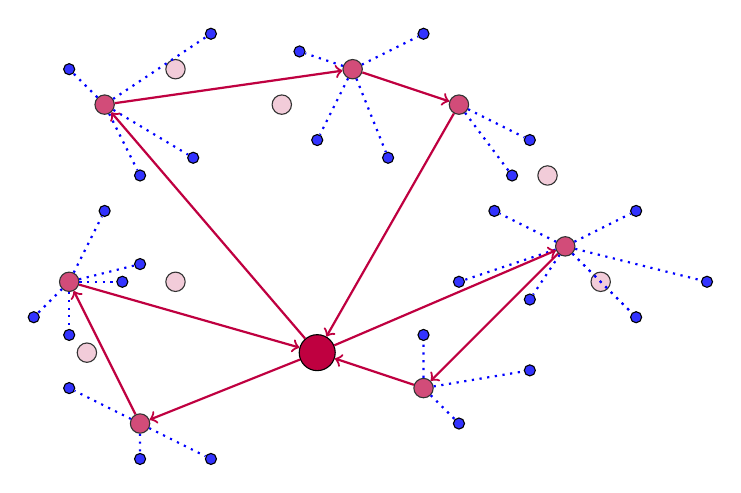
\begin{tikzpicture}[scale=0.45, auto,swap]
   		
   		\node[com2] (dum) at (0,5) {};
   		\node[j0] (j0) at (8,5) {};		
   		\node[com2] (be) at (19,5) { };
   		
   		
   		%%%%% Collection centers   (numerotes sens horaire)
   		\foreach \pos/\name/\denom in {{(3,3)/d1}, {(1,7)/d2},  {(2,12)/d3},  {(9,13)/d4}, {(12,12)/d5}, {(15,8)/d6}, {(11,4)/d7}}
   		\node[vertexD] (\name) at \pos {$ $};
   		
   		\foreach \pos/\name/\denom in {{(1.5,5)/d91}, {(4,7)/d92},  {(4,13)/d93},  {(7,12)/d94}, {(14.5,10)/d95}, {(16,7)/d96}}
   		\node[vertex0] (\name) at \pos {$ $};
   		
   		%%%% suppliers 
   		
   		\foreach \pos/\name/\denom in {{(1,4)/f11}, {(3,2)/f12}, {(5,2)/f13}}
   		\node[farm] (\name) at \pos {$ $};
   		
   		\foreach \pos/\name/\denom in {{(1,5.5)/f21}, {(2.5,7)/f22}, {(0,6)/f23}, {(3,7.5)/f24}, {(2,9)/f25}}
   		\node[farm] (\name) at \pos {$ $};
   		
   		\foreach \pos/\name/\denom in {{(4.5,10.5)/f31}, {(1,13)/f32}, {(5,14)/f33}, {(3,10)/f34}}
   		\node[farm] (\name) at \pos {$ $};
   		
   		\foreach \pos/\name/\denom in {{(8,11)/f41}, {(10,10.5)/f42}, {(11,14)/f43}, {(7.5,13.5)/f44}}
   		\node[farm] (\name) at \pos {$ $};
   		
   		
   		\foreach \pos/\name/\denom in {{(14,11)/f51}, {(13.5,10)/f52}}
   		\node[farm] (\name) at \pos {$ $};
   		
   		\foreach \pos/\name/\denom in {{(14,6.5)/f61}, {(12,7)/f62}, {(17,6)/f63}, {(19,7)/f64}, {(17,9)/f65}, {(13,9)/f66}}
   		\node[farm] (\name) at \pos {$ $};
   		
   		\foreach \pos/\name/\denom in {{(14,4.5)/f71}, {(12,3)/f72}, {(11,5.5)/f73}}
   		\node[farm] (\name) at \pos {$ $};
   		
   		
   		%%% Last mile
   		\foreach \source/ \dest in {d1/f11,d1/f12,d1/f13}	\path[edge1] (\source) -- (\dest) ;
   		\foreach \source/ \dest in {d2/f21,d2/f22,d2/f23,d2/f24,d2/f25}	\path[edge1] (\source) -- (\dest) ;
   		\foreach \source/ \dest in {d3/f31,d3/f32,d3/f33,d3/f34}	\path[edge1] (\source) -- (\dest) ;
   		\foreach \source/ \dest in {d4/f41,d4/f42,d4/f43,d4/f44}	\path[edge1] (\source) -- (\dest) ;
   		\foreach \source/ \dest in {d5/f51,d5/f52}	\path[edge1] (\source) -- (\dest) ;	
   		\foreach \source/ \dest in {d6/f61,d6/f62,d6/f63,d6/f63,d6/f64,d6/f65,d6/f66}	\path[edge1] (\source) -- (\dest) ;
   		\foreach \source/ \dest in {d7/f71,d7/f72,d7/f73}	\path[edge1] (\source) -- (\dest) ;
   		
   		%%%% Routes
   		\foreach \source/ \dest in {j0/d1,d1/d2,d2/j0}	\path[edgetr] (\source) -- (\dest) ;
   		\foreach \source/ \dest in {j0/d3,d3/d4,d4/d5,d5/j0} \path[edgetr] (\source) -- (\dest) ;
   		\foreach \source/ \dest in {j0/d6,d6/d7,d7/j0}	\path[edgetr] (\source) -- (\dest) ;
   		\end{tikzpicture}
   	\end{figure}
 
    	\subsection{New notation}
   	\begin{table}[htbp]
   		\begin{center}
   			\begin{tabular}{lp{12cm}}
   				\toprule
   				Data & Definition	\\
   				\addlinespace[2pt] 
   				\midrule
   				$R$							& Set of routes (in first layer) \\
    			$c_r$				& Cost of route $r \in R$ ($1^{st}$ layer)\\
   				$c'_{ij}$		& Cost of delivering customer $i\in I$ from DC $j \in J$  ($2^{nd}$ layer)\\ 
   				$\alpha_{jr}$		& =1 if route $r \in R$ visits DC $j \in J$, 0 otherwise \\
   				\bottomrule
   			\end{tabular}
   		\end{center}
     	\end{table}
   	
   	
   	\begin{table}[htbp]
   		\begin{center}
   			\begin{tabular}{lp{12cm}}
   				\toprule
   				\multicolumn{2}{l}{\textit{Binary Variables}} \\
   				\addlinespace[2pt]
   				$\textcolor{red}{y_j}$			& = 1 if distribution center $j \in J$ is selected. 0 otherwise.  \\
   				$\textcolor{orange}{z_r^t}$ 		& = 1 if route $r\in R$ is selected in period $t \in T$, 0 otherwise \\
   				$\textcolor{blue}{x_{ij}^t}$	& =1 if customer $i$ is delivered by DC $j \in J$ in time period $t \in T$ \\	
   				\midrule
   				\multicolumn{2}{l}{\textit{Continuous Variables}} \\
   				\addlinespace[2pt]
   				$v_{ij}^t$ 	& quantity delivered from DC $j \in J$ to customer $i \in I$ in period $t \in T$. \\
   				\bottomrule
   			\end{tabular}
   		\end{center}
    	\end{table}
    	
  
   	\subsection{LIRP model 2}
   	
  
   	\begin{equation}
   	\label{obj2}    	
   	\min 	\sum\limits_{j \in J} f_j \textcolor{red}{y_j}  
   	+ \sum\limits_{t \in T}  \left( \sum\limits_{j \in J} c_r \textcolor{orange}{z_r^t} 
   	+ \sum\limits_{i \in I}\sum\limits_{j \in J} c'_{ij} \textcolor{blue}{x_{ij}^t}  \right) 
   	+ \sum\limits_{t\in T}  \sum\limits_{i \in V^*} h_i^t I_i^t 
   	\end{equation}
   	
 \begin{align}
   &	\sum\limits_{r \in R} \alpha_{jr} \textcolor{orange}{z_r^t} \leq 1   	&& \forall j \in J, \forall t \in T \label{d02} \\
   &	q_j^t \leq Q \; \textcolor{orange}{z_r^t} && \forall j \in J, \forall r \in R, \forall t \in T \label{d03}\\
   &	\textcolor{orange}{z_r^t} \leq \alpha_{jr} \; \textcolor{red}{y_j} && \forall j \in J, \forall t \in T \label{d04}\\
   &	\sum\limits_{r\in R} \textcolor{orange}{z_r^t} \leq |K|  		&& \forall t \in T  \label{d05} \\
   &	v_{ij}^t \leq Q \;  \textcolor{blue}{x_{ij}^t} 	 && \forall i \in I,  \forall j \in J, \forall t \in T     \label{d06} \\
    &	v_{ij}^t\leq \left(\sum\limits_{t\geq t}^{t'\leq t+\tau_{max}}d_i^{t'}\right) \; \textcolor{blue}{x_{ij}^t}  && \forall i \in I, \forall j \in J, \forall t \in T \label{d07} \\
      &	\textcolor{blue}{x_{ij}^t} \leq \textcolor{red}{y_j} 	 && \forall i \in I,  \forall j \in J, \forall t \in T     \label{d08} 
 \end{align}
   	
 
 	
	
 	 \begin{align}
  &	I_j^t = I_j^{t-1} + q_j^t -  \sum\limits_{i \in I} v_{ij}^t  && \forall i \in I, \forall j \in J, \forall t \in T \label{c09} \\
  & 	I_i^t = I_i^{t-1} + \sum\limits_{j \in J} v_{ij}^t - d_i^t  && \forall i \in I, \forall t \in T \label{d10} \\ 
  & 	I_i^t \leq \sum\limits_{t'\geq t}^{t'\leq t+\tau_{max}} d_i^{t'}  && \forall i \in I, \forall t \in T \label{d11} \\
  & 	\textcolor{red}{y_j} \in \{0,1\} && \forall j \in J \\
  & 	\textcolor{orange}{z_r^t} \in \{0,1\} && \forall r \in R, \forall t \in T \\
  & 	\textcolor{blue}{x_{ij}^t} \in \{0,1\} && \forall i \in I, \forall j \in J, \forall t \in T \\
  & 	I_i^t, I_j^t \geq 0	&&  \forall i\in I, \forall j\in J, \forall t \in T \\
  & 	q_j^t,v_{ij}^t \geq 0  && \forall i\in I, \forall j\in J, \forall t \in T, \forall r \in R
   	\end{align}
  
	\subsection{Constraints of model 2 (v�rifier num�rso �quations)}
   	\begin{itemize} 
   		\item Objective function = facility fixed cost + routing cost + inventory cost
   		\item  (21) Each DC is visited by at most one route in every time period
   		\item  (22) Capacity constraint on routes.
   		\item (23) No routes to unselected distribution centers
   		\item (24) Fleet size limitation
   	   	\item  (25) (22) Capacity constraints on route $r$, if it is performed in time period $t$.
   	   	\item (26) A customer is served from a selected distribution center
    	\item  (27) Flow conservation at DC $j$
   		\item (28) Flow conservation at customer $i$
   		\item  (29) Max inventory at customers (valid inequality)
   	\end{itemize}
  
 	 
 	   	
 	   	

   
  
  
\end{document}

